\chapter[Metodologia]{Metodologia}

\section{Metodologia de Desenvolvimento}

Para o desenvolvimento do trabalho será adotada uma metodologia híbrida, contendo diferentes ferramentas de abordagens de desenvolvimento de software. Essa personalização tem o objetivo de otimizar o desenvolvimento das tarefas no contexto em que esse trabalho é desenvolvido, tendo como uma das motivações principais para realizar essa personalização o fato do trabalho não ser construído em grupo.

Será utilizada a metodologia KanBan, com algumas personalizações, para gerenciar a execução de atividades. Os cartões utilizados neste quadro estarão representados no formato de \textit{User Story}, comumente utilizada na metodologia SCRUM, com seu conteúdo sendo composto por: uma descrição no formato da sentença \textbf{Eu como <quem>, quero <o que>, para <ação>}, as \textit{tasks} a serem desenvolvidas, o tempo limite para sua realização e a categoria da mesma.

O quadro será composto por 4 diferentes colunas: A fazer, Fazendo, Aguardando Validação e Finalizados. A imagem a seguir exemplifica o fluxo de desenvolvimento no quadro \textit{KanBan} que será utilizado no trabalho.

    \begin{figure}[H]
         \centering
         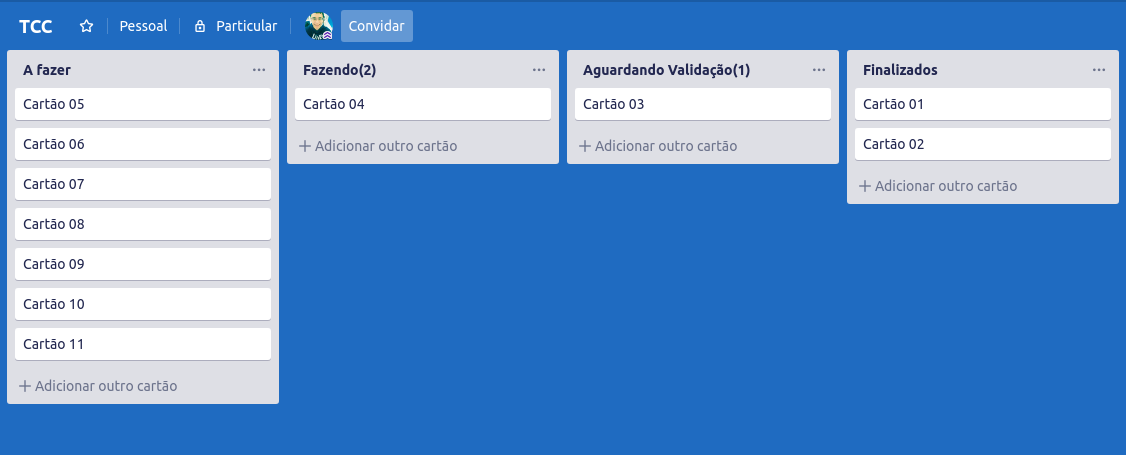
\includegraphics[scale=0.4]{figuras/capitulo_4/kanban_exemplo.png}
         \caption{KanBan representado na ferramenta \href{https://trello.com/}{Trello}}
         \label{fig:kanban_trello_exe}
    \end{figure}

A coluna \textbf{A Fazer} funcionará como um \textit{Backlog} das funcionalidades que serão desenvolvidas ao decorrer do trabalho (possíveis \textit{bugs} ou melhorias que surjam ao decorrer do projeto também serão adicionadas à essa coluna), onde os cartões posicionados acima são os considerados de maior prioridade para serem desenvolvidos. A coluna \textbf{Fazendo} será responsável por indicar o cartão que está que está em processo de desenvolvimento. Já a \textbf{Aguardando Validação} indicará o cartão que está passando por um processo de validação, como por exemplo a realização de testes com usuários reais para validar o funcionamento implementado em relação ao descrito no cartão. E a coluna \textbf{Finalizados} conterá o histórico das funcionalidades já implementadas e que foram validadas de acordo com os testes planejados.

Para melhor monitorar o andamento do trabalho, o planejamento dos cartões será feito por meio de iterações semanais. Neste planejamento semanal poderão ocorrer mudanças nas prioridades dos cartões presentes no quadro \textit{KanBan}, inserção de novos cartões na fila \textbf{A fazer}, remoção do quadro cartões que são considerados não necessários ou que precisem ser desmembrados em outros cartões pela complexidade da atividade. 

\section{Políticas para o desenvolvimento do Projeto}

Toda a aplicação terá sua construção feita na plataforma \href{https://github.com/}{GitHub}
em um repositório fechado. As issues do GitHub serão utilizadas como os cartões do KanBan para o cadastro das informações necessárias, e serão gerenciados de forma visual por meio da ferramenta \href{https://www.zenhub.com/}{ZenHub}.
 
A cada adição de funcionalidade ao sistema um novo \textit{commit} será feito para um melhor versionamento e controle do que será desenvolvido, e cada \textit{commit} terá seu texto no padrão \textbf{\#IdDaIssue Descrição}, como no seguinte caso:  “\#1 - Creating user structure”.

O repositório do projeto contará com duas branches principais para o desenvolvimento, sendo elas: \textit{master} e \textit{devel}. A branch \textit{master} conterá a versão estável do projeto, tendo seu conteúdo proveniente da branch de desenvolvimento (\textit{devel}), que será utilizada para o desenvolvimento do projeto, após a validação do que foi desenvolvido. Por decisões de projeto, nenhum \textit{commit} poderá ser feito diretamente na \textit{branch} \textit{master}, onde para inserir novos arquivos deve ser realizado um \textit{merge/pull request} tendo como origem das informações a \textit{branch devel}.



\section{Cronograma}

O cronograma a seguir apresenta as atividades que foram realizadas durante ao período correspondente ao TCC 1 e também apresenta as atividades que serão realizadas para o desenvolvimento deste
trabalho no período que corresponde ao TCC 2. As atividades são:

    \begin{enumerate}
        \item Estudo sobre a tecnologia Blockchain;
        \item Estudo do uso de aplicações descentralizadas em contextos diversos;
        \item Estudo sobre a regulamentação de trânsito referente a problemática que será estudada;
        \item Desenhar uma arquitetura inicial para a aplicação;
        \item Redigir o texto correspondente ao TCC 1;
        \item Apresentação do TCC 1;
        \item Desenvolver a aplicação;
        \item Realizar testes para validar a aplicação desenvolvida;
        \item Redigir o texto correspondente ao TCC 2;
        \item Apresentação do TCC 2;
    \end{enumerate}
    
    
Para uma melhor visualização das atividades, as mesmas serão dividas em duas tabelas. A Tabela \ref{tabela_cronograma_tcc1} contém o cronograma das atividades desempenhadas no período do TCC 1, e a Tabela \ref{tabela_cronograma_tcc2} corresponde ao planejamento inicial das atividades que serão realizadas no período do TCC 2.

    
    \begin{table}[H]
        \caption{Cronograma TCC 1.}
        \begin{adjustbox}{width=\textwidth}
            \begin{tabular}{|l|c|c|c|c|c|}
            \hline
            \multicolumn{1}{|c|}{\textbf{}} & \textbf{Março} & \multicolumn{1}{l|}{\textbf{Abril}} & \multicolumn{1}{l|}{\textbf{Maio}} & \multicolumn{1}{l|}{\textbf{Junho}} & \multicolumn{1}{l|}{\textbf{Julho}} \\ \hline
            Estudo sobre a tecnologia Blockchain & X & X & X &  &  \\ \hline
            Estudo do uso de aplicações descentralizadas em contextos diversos &  & X &  &  &  \\ \hline
            Estudo sobre a regulamentação de trânsito referente a problemática que será estudada &  & X &  &  &  \\ \hline
            Desenho de uma arquitetura inicial para a aplicação &  &  & X &  &  \\ \hline
            Redigir o texto correspondente ao TCC 1 &  & X & X & X &  \\ \hline
            Apresentação do TCC 1 &  &  &  &  & X \\ \hline
            \end{tabular}
        \end{adjustbox}
        \label{tabela_cronograma_tcc1}
    \end{table}

    \begin{table}[H]
        \caption{Cronograma TCC 2.}
        \begin{adjustbox}{width=\textwidth}    
            \begin{tabular}{|l|c|c|c|c|c|}
            \hline
            \multicolumn{1}{|c|}{\textbf{}} & \textbf{Agosto} & \multicolumn{1}{l|}{\textbf{Setembro}} & \multicolumn{1}{l|}{\textbf{Outubro}} & \multicolumn{1}{l|}{\textbf{Novembro}} & \multicolumn{1}{l|}{\textbf{Dezembro}} \\ \hline
            Desenvolver a aplicação & X & X & X &  &  \\ \hline
            Realizar testes para validar a aplicação desenvolvida &  & X & X & X &  \\ \hline
            Redigir o texto correspondente ao TCC 2 &  &  & X & X &  \\ \hline
            Apresentação do TCC 2 &  &  &  &  & X \\ \hline
            \end{tabular}
        \end{adjustbox}
        \label{tabela_cronograma_tcc2}
    \end{table}